\documentclass[12pt]{article}

\usepackage{tabularx}
\usepackage[a4paper,margin=2.5cm, bottom=3.5cm]{geometry}
\usepackage{fancyhdr}
\usepackage{listings}
\usepackage{booktabs}
\usepackage{float}
\usepackage{subcaption}
\usepackage{graphicx}
\usepackage{amsmath}
\usepackage{amssymb}
\usepackage{amsthm}
\usepackage{array}
\usepackage[table]{xcolor}
\usepackage{pgfplots}
\usepackage{pgfplotstable}
\usepackage{multirow}
\usepackage{tikz}
\usepackage[hidelinks]{hyperref}
\usepackage{titling}
\pgfplotsset{compat=1.17}

\theoremstyle{definition}
\newtheorem*{example}{Example}
\setlength{\headheight}{40pt}
\setlength{\parindent}{0pt}
\setlength{\parskip}{1ex}
\renewcommand{\headrulewidth}{0pt}

\newcommand{\subfiguresize}{.3\textwidth}
\DeclareMathOperator*{\median}{median}

\DeclareMathOperator*{\biggerforall}{\mbox{\Large $\mathsurround0pt\forall$}} 
\DeclareMathOperator*{\bigforall}{\mbox{\large $\mathsurround0pt\forall$}} 
\DeclareMathOperator*{\biggerexists}{\mbox{\Large $\mathsurround0pt\exists$}} 
\DeclareMathOperator*{\bigexists}{\mbox{\large $\mathsurround0pt\exists$}} 

\lstset {
    captionpos = b,
    basicstyle = \small\ttfamily,
    keywordstyle = \color{blue},
    commentstyle = \color{black!30},
    comment = [l]{//},
    morecomment = [s]{/*}{*/},
    identifierstyle=,
    keywords = {
        let,
        mut,
        for,
        in,
        if,
        else,
        continue,
        break,
        pub,
        struct,
        impl,
        type,
        self,
        Self,
        as,
        u8,u16,u32,u64,
        i8,i16,i32,i64,
        f32,f64,
        usize,
    }
}

\pagestyle{fancy}
\fancyhead{}
\fancyhead[L]{
    \renewcommand{\arraystretch}{1.5}
    \begin{tabularx}{\textwidth}{|X|X|}
        \hline
        \large \bf Image processing & \normalsize \thetitle \\
        \hline
    \end{tabularx}
}
\fancyfoot[C]{\thepage}

\renewcommand{\maketitle}{
    \thispagestyle{plain}
    \renewcommand{\arraystretch}{2}
    \vspace*{-7em}
    \begin{flushleft}
        \begin{tabularx}{0.95\textwidth}{|X|X|}
            \hline
            \bf \large Image Processing                   & \bf \large \thetitle                           \\ \hline
            \multicolumn{2}{|l|}{
                \textbf{Task variant:} Group 1
            }                                                                                               \\ \hline
            \textbf{Day and time:} Mon, 14:00             & \textbf{Full name:} \textsc{Jakub Pawlak}       \\
            \textbf{Academic year:} {2022/23} & \textbf{Full name:} \textsc{Magdalena Paku\l a} \\
            \hline
        \end{tabularx}
    \end{flushleft}
    \vspace{1em}
    \renewcommand{\arraystretch}{1}
}
\renewcommand{\subfiguresize}{.25\textwidth}
\graphicspath{{img},{../img}}

\usetikzlibrary{matrix}
\tikzset{square matrix/.style={
    matrix of nodes,
    nodes in empty cells,
    column sep=-\pgflinewidth, row sep=-\pgflinewidth,
    nodes={draw,
      minimum height=#1,
      anchor=center,
      text width=#1,
      align=center,
      inner sep=0pt
    },
  },
  square matrix/.default=1.5em
}

\title{Task No.~3}

\begin{document}
\maketitle

\section{Description of the implementation of the basic \texorpdfstring{\\ }{} morphological operations}

\subsection*{Optimization}

To make operations on binary images more efficient,
we represent the binary mask not as an image or collection of coordinates,
but as a slice of memory where each bit corresponds to a specific pixel.
This is done to firstly reduce the memory size, and secondly to make the operations faster by enabling the use of
binary operators, which are $\mathcal{O}(1)$.

Since the mask is a finite cartesian coordinate plane, we can assign each point $(x,y)$,
a unique number $n = x + wy$, where $w$ is the width of the coordinate plane.
The pixel will be assigned the $n$-th bit.

Therefore, for a $3\times3$ mask, it will be represented in the following way

\begin{center}
    \begin{tikzpicture}[baseline=(Center.base)]
        \matrix[square matrix]
        {
        |[fill=gray]| & |[fill=gray]| & \\
        & |(Center)[fill=gray]| & \\
        & & |[fill=gray]| \\
        };
    \end{tikzpicture}
    $\; \Longleftrightarrow \; (100010011)_2$
\end{center}

The struct to hold the data is implemented as the following:

\begin{lstlisting}
#[derive(Clone, Eq, PartialEq)]
pub struct Mask {
    data: u16,
}
\end{lstlisting}

Note that we use \lstinline{u16}, because for a $3\times3$ element, we only need 9 bits, so 2 bytes.
Our implementation currently suppports $3\times3$ structuring elements only, however, it would be very easy to extend for bigger elemens, as all the operations happen internally inside this struct,
so the implementations of the morphological operations would not need to be changed.

However, since the input is in the image form, we need a function to convert between the image and binary representations.
This function will take the image, as well as a set of $(x,y)$ coordinates, and construct the mask from the pixels neighboring $(x,y)$.

\begin{equation}
    \mathbf{M}(A,x,y) \to B
\end{equation}

\begin{center}
    \begin{tikzpicture}[baseline=(Center.base)]
        \matrix[square matrix=1em]
        {
        |[fill=gray]|&&|[fill=gray]|&&|[fill=gray]|\\
        |[fill=gray]|&|[fill=gray]| & |[fill=gray]| && \\
        && |(Center)[fill=gray]|{$\bullet$} && \\
        && & |[fill=gray]| &|[fill=gray]| \\
        &|[fill=gray]|&|[fill=gray]|&&|[fill=gray]|\\
        };
    \end{tikzpicture}
    $\; \mapsto \; $
    \begin{tikzpicture}[baseline=(Center.base)]
        \matrix[square matrix=1em]
        {
        |[fill=gray]| & |[fill=gray]| & \\
        & |(Center)[fill=gray]| & \\
        & & |[fill=gray]| \\
        };
    \end{tikzpicture}
\end{center}


\begin{lstlisting}
pub fn from_image(image: &GrayImage, x: u32, y: u32) -> Mask {
    let mut mask = Mask::new();
    for i in 0..3 {
        for j in 0..3 {
            if is_unwritable(image, x, y, i, j) {
                continue;
            }
            mask.set_pixel(
                i, 
                j, 
                image.get_pixel(x + i - 1, y + j - 1)
            );
        }
    }
    mask
}
\end{lstlisting}

\vspace{2em}
We have also implemented the reverse function,
to set the pixels in the image from the binary implementation.

\begin{lstlisting}
pub fn write_to_image(
    &self, 
    image: &mut GrayImage, 
    x: u32, 
    y: u32
) {
    for i in 0..3 {
        for j in 0..3 {
            if is_unwritable(image, x, y, i, j) {
                continue;
            }
            image.put_pixel(
                x + i - 1, 
                y + j - 1, 
                self.get_pixel(i, j)
            );
        }
    }
}
\end{lstlisting}

Note that this function,
will overwrite the existing pixels if they are foreground in image,
but background in mask.

\pagebreak[4]
\subsection{Dilation}

The dilation of a binary image $A$ by a binary mask $B$ is defined as
\begin{equation}
    A \oplus B = \bigcup_{a \in A} B_a
\end{equation}

\begin{center}
    \begin{tikzpicture}[baseline=(A.base)]
        \matrix[square matrix]
        {
        &&\\
        &|(A)[fill=gray]|&|[fill=gray]|\\
        |[fill=gray]|&|[fill=gray]|&\\
        };
    \end{tikzpicture}
    $\; \oplus \; $
    \begin{tikzpicture}[baseline=(A.base)]
        \matrix[square matrix]
        {
        & |[fill=gray]| & \\
        & |[fill=gray]|$\odot$ & \\
        & &  \\
        };
    \end{tikzpicture}
    $\; = \; $
    \begin{tikzpicture}[baseline=(A.base)]
        \matrix[square matrix]
        {
        &|[fill=gray]|&|[fill=gray]|\\
        |[fill=gray]|&|[fill=gray]|&|[fill=gray]|\\
        |[fill=gray]|&|[fill=gray]|&\\
        };
    \end{tikzpicture}
\end{center}

To calculate the dilation of image $A$ by mask $B$,
we first need to allocate a new image $A'$.
This is done, because the dilation operating on more than one pixel,
so we cannot corrupt the original data.

Then, for each pixel $(x,y) \in A$, if $A(x,y)$ is foreground,
we perform the folliwing steps:
\begin{enumerate}
    \item Convert the neighbourhood of $(x,y)$ from $A'$ to binary mask $B'$
    \item Apply the binary or operation to the acquired mask and the mask $B$
    \item Save the result to the image $A'$
\end{enumerate}

\begin{lstlisting}
for (x, y, pixel) in image.enumerate_pixels() {
    if !is_foreground(pixel) {
        continue;
    }
    let new_image_mask = Mask::from_image(&new_image, x, y);
    let mask = self.mask | new_image_mask;
    mask.write_to_image(&mut new_image, x, y);
}
\end{lstlisting}

\subsection{Erosion}

Erosion of $A$ by $B$ is defined as
\begin{equation}
    A \ominus B = \left\{ (x,y) \mid B_{(x,y)} \subseteq A \right\}
    \label{eq:erosion-formal-def}
\end{equation}

\begin{center}
    \begin{tikzpicture}[baseline=(A.base)]
        \matrix[square matrix]
        {
        &&|[fill=gray]|\\
        &|(A)[fill=gray]|&|[fill=gray]|\\
        |[fill=gray]|&|[fill=gray]|&\\
        };
    \end{tikzpicture}
    $\; \ominus \; $
    \begin{tikzpicture}[baseline=(A.base)]
        \matrix[square matrix]
        {
        & |[fill=gray]| & \\
        & |[fill=gray]|$\odot$ & \\
        & &  \\
        };
    \end{tikzpicture}
    $\; = \; $
    \begin{tikzpicture}[baseline=(A.base)]
        \matrix[square matrix]
        {
        &&\\
        &&|[fill=gray]|\\
        &|[fill=gray]|&\\
        };
    \end{tikzpicture}
\end{center}

We can check the condition that $B_{(x,y)} \subseteq A$ very easily by usin the binary and operation.
\begin{equation}
    B_{(x,y)} \subseteq A \;\Leftrightarrow\; B = \left( B \land \mathbf{M}(A,x,y) \right)
\end{equation}

\pagebreak[2]
We can thus rewrite eq. (\ref{eq:erosion-formal-def}) as:
\begin{equation}
    A \ominus B = \left\{ (x,y) \mid B = \big( B \land \mathbf{M}(A,x,y) \big) \right\}
\end{equation}


Therefore, to calculate $A \ominus B$, for each $(x,y) \in A$, we perform the following steps:
\begin{enumerate}
    \item Convert the neighbourhood of $(x,y)$ from $A$ to binary form
    \item Apply the binary and operation to the acquired mask and the mask $B$
    \item If the result of the prevous step is equal to $B$, we set $A'(x,y)$ to foreground
\end{enumerate}

\pagebreak[3]
\begin{lstlisting}
for (x, y, pixel) in image.enumerate_pixels() {
    let mask = self.mask & Mask::from_image(&image, x, y);
    if mask == self.mask {
        new_image.put_pixel(x, y, FOREGROUND_PIXEL);
    }
}
\end{lstlisting}

\subsection{Opening}
The opening is simply defined as applying opening after erosion with the same kernel.
The erosion operation removes small elements from the image, 
while the dilation operation expands the remaining elements. 

The formal definition of this operation is:

\begin{equation}
   A \circ B  = ( A \ominus B )\oplus B
\end{equation}

Below is the implementation we used in the project.
\begin{lstlisting}
impl MorphologicalTransform for Opening {
    fn apply_morph_operation(&self, image: &mut GrayImage) {
        Erosion::apply(&self.mask, image);
        Dilation::apply(&self.mask, image);
    }
}
\end{lstlisting}

\subsection{Closing}

The closing operation is performed by first dilating the image and then eroding it. 
This has the effect of ``closing'' small gaps or holes within an object, 
and can be useful for smoothing out noise or filling in small defects in an image. 
It can also be used to extract specific features from an image, 
such as blobs or connected components, by removing small, 
isolated pixels or structures that do not contribute to the overall shape of the object.

\pagebreak[2]
The formal definition of this operation is:

\begin{equation}
   A \bullet B  = ( A \oplus B )\ominus B
\end{equation}

\pagebreak[2]
Below is the implementation we used in the project.
\begin{lstlisting}
impl MorphologicalTransform for Closing {
    fn apply_morph_operation(&self, image: &mut GrayImage) {
        Dilation::apply(&self.mask, image);
        Erosion::apply(&self.mask, image);
    }
}
\end{lstlisting}

\subsection{Hit-or-miss transform}

The \textsc{hmt} of $A$ with $\mathbf{B}$ where $\mathbf{B} = (B_{hit},B_{miss})$, is defined as
\begin{equation}
    A \otimes \mathbf{B} = \left\{ p \mid \biggerforall\limits_{\substack{b_{hit} \in B_{hit} \\ b_{miss} \in B_{miss}}}\; p + b_{hit} \in A \land p + b_{miss} \notin A  \right\}
\end{equation}

\begin{center}
    \begin{tikzpicture}[baseline=(A.base)]
        \matrix[square matrix]
        {
        &&|[fill=gray]|&&\\
        &|[fill=gray]|&&|[fill=gray]|&\\
        &|[fill=gray]|&|(A)[fill=gray]|&|[fill=gray]|&\\
        &|[fill=gray]|&&|[fill=gray]|&\\
        &&&&\\
        };
    \end{tikzpicture}
    $\; \ominus \; $
    \begin{tikzpicture}[baseline=(A.base)]
        \matrix[square matrix]
        {
        & |[fill=green]| & \\
        & $\odot$ & |[fill=red]| \\
        & &|[fill=red]|  \\
        };
    \end{tikzpicture}
    $\; = \; $
    \begin{tikzpicture}[baseline=(A.base)]
        \matrix[square matrix]
        {
        &&&&\\
        &&&&\\
        &&&|[fill=gray]|&\\
        &|[fill=gray]|&&|[fill=gray]|&\\
        &|[fill=gray]|&&|[fill=gray]|&\\
        };
    \end{tikzpicture}
\end{center}

However, for our implementation, we will use the following property:
\begin{equation}
    A \otimes \mathbf{B} = (A \ominus B_1) \cap (A^C \ominus B_2)
\end{equation}

Which we can rewrite to make use of the binary operators as the following:

\begin{equation}
    A \otimes \mathbf{B} = \left\{ (x,y) \mid
    \Big(B_1 = \big(B_1 \land \mathbf{M}(A,x,y)\big)\Big)
    \land \Big( B_2 = \big( B_2 \land \neg \mathbf{M}(A,x,y) \big) \Big)
    \right\}
\end{equation}

The core of our \textsc{hmt} transform implementation is a helper function \lstinline{get_matching_pixels}, which operates on an iterator.
It takes a reference to the image, and outputs the $(x,y)$ coordinates of the pixels that fullfill the conditions of the \textsc{hmt}.

We could just use a for-loop and check the condition inside of it, however,
a helper function operating on an iterator will prove to be very useful when implementing the convex hull in section \ref{sec:convex-hull-impl}.

\pagebreak[2]
The function is implemented in the following way:

\begin{lstlisting}
pub(crate) fn get_matching_pixels<'img, 's, 'out>(
    &'s self,
    image: &'img GrayImage,
) -> impl Iterator<Item = (u32, u32)> + 'out
where
    'img: 'out,
    's: 'out
{
    image
      .enumerate_pixels()
      .map(|(x, y, _)| (x, y)) // discard the pixel reference
      .filter(|(x, y)| {
          let img_mask = &Mask::from_image(image, *x, *y);
          let is_hit = 
            self.hit_mask == (&self.hit_mask & img_mask);
          let is_miss = 
            self.miss_mask == (&self.miss_mask & &(!img_mask));  
          
          is_hit && is_miss
      })
}
\end{lstlisting}

\begin{remark}
    Although the function signature might look a bit intimidating due to annotations such as \lstinline{'img}, \lstinline{'s}, and \lstinline{'out},
    it is actually very straightforward.
    These are so-called \emph{lifetime annotations} that helps the rust compiler ensure the memory safety at compile time.
    Since the function result operates on the data from the image, and the \textsc{hmt} struct holding the structring elements,
    we have to constraint the lifetime of the result, such that the \textsc{hmt} struct and the image both have to be valid for at least
    as long as the result of the function.
\end{remark}

Finally, the implementation of the \textsc{hmt} is very straightforward, we just allocate a buffer for the new image
and set all the pixels that match the \textsc{hmt} conditions as foreground.

\begin{lstlisting}
let mut new_image: GrayImage = /* ... */
for (x, y) in self.get_matching_pixels(image) {
    new_image.put_pixel(x, y, FOREGROUND_PIXEL);
}
*image = new_image;
\end{lstlisting}

\pagebreak[2]
\section{Analysis of the results of the basic morphological operations}

\begin{figure}[H]\centering
    \begin{subfigure}[t]{.2\textwidth}\centering
        \begin{tikzpicture}
            \matrix[square matrix]
            {
            &&\\
            &|[fill=gray]|$\odot$&|[fill=gray]|\\
            &&\\
            };
        \end{tikzpicture}
        \caption{$B_1$}
    \end{subfigure}
    \begin{subfigure}[t]{.2\textwidth}\centering
        \begin{tikzpicture}
            \matrix[square matrix]
            {
            &&\\
            &|[fill=gray]|$\odot$&\\
            &|[fill=gray]|&\\
            };
        \end{tikzpicture}
        \caption{$B_2$}
    \end{subfigure}
    \begin{subfigure}[t]{.2\textwidth}\centering
        \begin{tikzpicture}
            \matrix[square matrix]
            {
            |[fill=gray]|&|[fill=gray]|&|[fill=gray]|\\
            |[fill=gray]|&|[fill=gray]|$\odot$&|[fill=gray]|\\
            |[fill=gray]|&|[fill=gray]|&|[fill=gray]|\\
            };
        \end{tikzpicture}
        \caption{$B_3$}
    \end{subfigure}
    \begin{subfigure}[t]{.2\textwidth}\centering
        \begin{tikzpicture}
            \matrix[square matrix]
            {
            &|[fill=gray]|&\\
            |[fill=gray]|&|[fill=gray]|$\odot$&|[fill=gray]|\\
            &|[fill=gray]|&\\
            };
        \end{tikzpicture}
        \caption{$B_4$}
    \end{subfigure}
    \caption{Kernels used for testing}
\end{figure}

\subsection{Dilation}

The result of running dilation with different kernels are presented below.
The operation seems to behave correctly,
adding pixels to the image exactly as expected.

As the morphological operations are very simple, there is not much possibility for conclusions.

The only remark that comes to head is that the shape of the kernel greately influences the shape of the output,
namely kernel $B_3$ is very ``blocky'' and so are the results of applying it, whereas $B_4$ and its outputs are more ``round''.

\begin{figure}[H]\centering
    \begin{subfigure}[t]{\subfiguresize}\centering
        
\includegraphics[width=\textwidth]{img/image1.png}
        \caption{before}
    \end{subfigure}
    \hspace{2em}
    \begin{subfigure}[t]{\subfiguresize}\centering
        
\includegraphics[width=\textwidth]{img/image1-dilation-b1.png}
        \caption{after}
    \end{subfigure}\\[1em]
    \begin{subfigure}[t]{\subfiguresize}\centering
        
\includegraphics[width=\textwidth]{img/image2.png}
        \caption{before}
    \end{subfigure}
    \hspace{2em}
    \begin{subfigure}[t]{\subfiguresize}\centering
        
\includegraphics[width=\textwidth]{img/image2-dilation-b1.png}
        \caption{after}
    \end{subfigure}
    \caption{Results of applying dilation with kernel $B_1$}
\end{figure}   

\begin{figure}[H]\centering
    \begin{subfigure}[t]{\subfiguresize}\centering
        
\includegraphics[width=\textwidth]{img/image1.png}
        \caption{before}
    \end{subfigure}
    \hspace{2em}
    \begin{subfigure}[t]{\subfiguresize}\centering
        
\includegraphics[width=\textwidth]{img/image1-dilation-b2.png}
        \caption{after}
    \end{subfigure}\\[1em]
    \begin{subfigure}[t]{\subfiguresize}\centering
        
\includegraphics[width=\textwidth]{img/image2.png}
        \caption{before}
    \end{subfigure}
    \hspace{2em}
    \begin{subfigure}[t]{\subfiguresize}\centering
        
\includegraphics[width=\textwidth]{img/image2-dilation-b2.png}
        \caption{after}
    \end{subfigure}
    \caption{Results of applying dilation with kernel $B_1$}
\end{figure}  

\begin{figure}[H]\centering
    \begin{subfigure}[t]{\subfiguresize}\centering
        
\includegraphics[width=\textwidth]{img/image1.png}
        \caption{before}
    \end{subfigure}
    \hspace{2em}
    \begin{subfigure}[t]{\subfiguresize}\centering
        
\includegraphics[width=\textwidth]{img/image1-dilation-8adj.png}
        \caption{after}
    \end{subfigure}\\[1em]
    \begin{subfigure}[t]{\subfiguresize}\centering
        
\includegraphics[width=\textwidth]{img/image2.png}
        \caption{before}
    \end{subfigure}
    \hspace{2em}
    \begin{subfigure}[t]{\subfiguresize}\centering
        
\includegraphics[width=\textwidth]{img/image2-dilation-8adj.png}
        \caption{after}
    \end{subfigure}
    \caption{Results of applying dilation with kernel $B_3$}
\end{figure}    

\begin{figure}[H]\centering
    \begin{subfigure}[t]{\subfiguresize}\centering
        
\includegraphics[width=\textwidth]{img/image1.png}
        \caption{before}
    \end{subfigure}
    \hspace{2em}
    \begin{subfigure}[t]{\subfiguresize}\centering
        
\includegraphics[width=\textwidth]{img/image1-dilation-4adj.png}
        \caption{after}
    \end{subfigure}\\[1em]
    \begin{subfigure}[t]{\subfiguresize}\centering
        
\includegraphics[width=\textwidth]{img/image2.png}
        \caption{before}
    \end{subfigure}
    \hspace{2em}
    \begin{subfigure}[t]{\subfiguresize}\centering
        
\includegraphics[width=\textwidth]{img/image2-dilation-4adj.png}
        \caption{after}
    \end{subfigure}
    \caption{Results of applying dilation with kernel $B_4$}
\end{figure} 

\begin{figure}[H]\centering
    \begin{subfigure}[t]{\subfiguresize}\centering
        \fbox{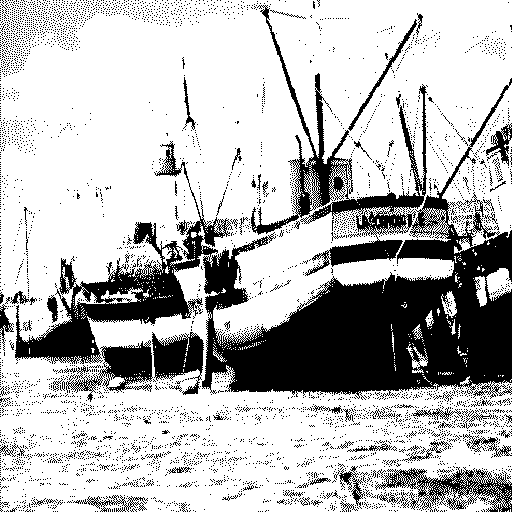
\includegraphics[width=.9\textwidth]{img/boat.png}}
        \caption{original}
    \end{subfigure}
    \hspace{2em}
    \begin{subfigure}[t]{\subfiguresize}\centering
        \fbox{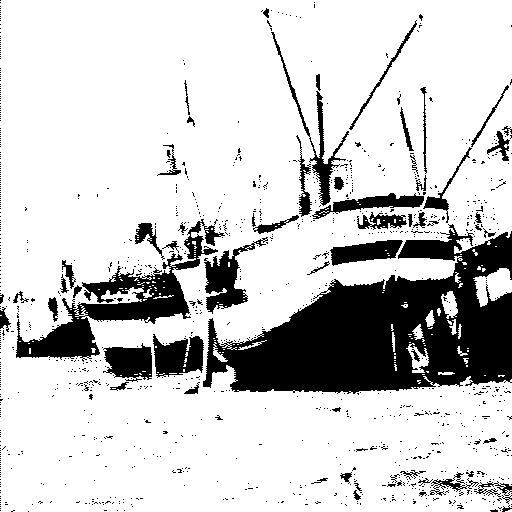
\includegraphics[width=.9\textwidth]{img/boat-dilation-b1.png}}
        \caption{$B_1$}
    \end{subfigure}
    \hspace{2em}
    \begin{subfigure}[t]{\subfiguresize}\centering
        \fbox{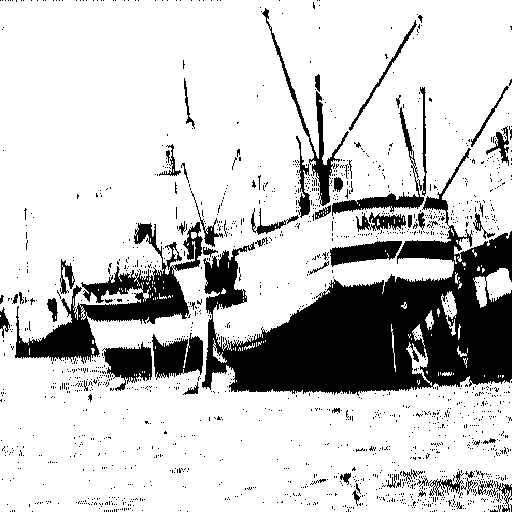
\includegraphics[width=.9\textwidth]{img/boat-dilation-b2.png}}
        \caption{$B_2$}
    \end{subfigure}\\[1em]
    \hspace{2em}
    \begin{subfigure}[t]{\subfiguresize}\centering
        \fbox{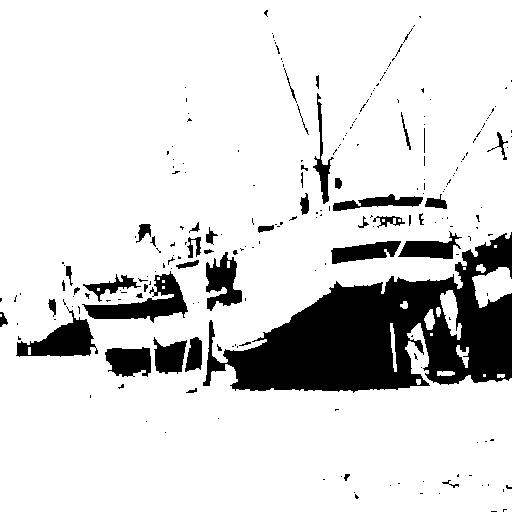
\includegraphics[width=.9\textwidth]{img/boat-dilation-b3.png}}
        \caption{$B_3$}
    \end{subfigure}
    \hspace{2em}
    \begin{subfigure}[t]{\subfiguresize}\centering
        \fbox{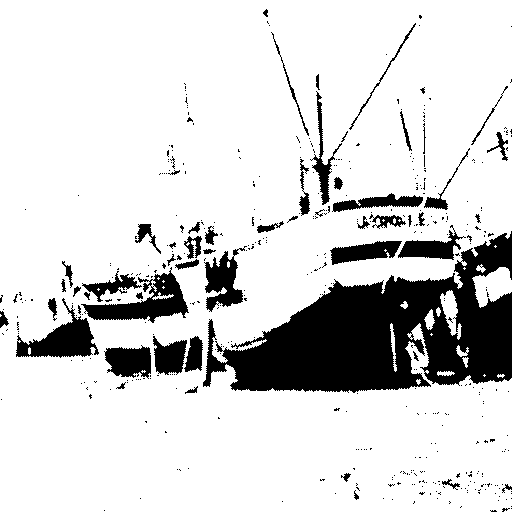
\includegraphics[width=.9\textwidth]{img/boat-dilation-b4.png}}
        \caption{$B_4$}
    \end{subfigure}
    \hspace{2em}
    \caption{Results of applying dilation on the boat image}
\end{figure} 

\subsection{Erosion}

\begin{figure}[H]\centering
    \begin{subfigure}[t]{\subfiguresize}\centering
        
\includegraphics[width=\textwidth]{img/image1.png}
        \caption{before}
    \end{subfigure}
    \hspace{2em}
    \begin{subfigure}[t]{\subfiguresize}\centering
        
\includegraphics[width=\textwidth]{img/image1-erosion-b1.png}
        \caption{after}
    \end{subfigure}\\[1em]
    \begin{subfigure}[t]{\subfiguresize}\centering
        
\includegraphics[width=\textwidth]{img/image2.png}
        \caption{before}
    \end{subfigure}
    \hspace{2em}
    \begin{subfigure}[t]{\subfiguresize}\centering
        
\includegraphics[width=\textwidth]{img/image2-erosion-b1.png}
        \caption{after}
    \end{subfigure}
    \caption{Results of erosion dilation with kernel $B_1$}
\end{figure} 

\begin{figure}[H]\centering
    \begin{subfigure}[t]{\subfiguresize}\centering
        
\includegraphics[width=\textwidth]{img/image1.png}
        \caption{before}
    \end{subfigure}
    \hspace{2em}
    \begin{subfigure}[t]{\subfiguresize}\centering
        
\includegraphics[width=\textwidth]{img/image1-erosion-b2.png}
        \caption{after}
    \end{subfigure}\\[1em]
    \begin{subfigure}[t]{\subfiguresize}\centering
        
\includegraphics[width=\textwidth]{img/image2.png}
        \caption{before}
    \end{subfigure}
    \hspace{2em}
    \begin{subfigure}[t]{\subfiguresize}\centering
        
\includegraphics[width=\textwidth]{img/image2-erosion-b2.png}
        \caption{after}
    \end{subfigure}
    \caption{Results of erosion dilation with kernel $B_2$}
\end{figure} 

\begin{figure}[H]\centering
    \begin{subfigure}[t]{\subfiguresize}\centering
        
\includegraphics[width=\textwidth]{img/image1.png}
        \caption{before}
    \end{subfigure}
    \hspace{2em}
    \begin{subfigure}[t]{\subfiguresize}\centering
        
\includegraphics[width=\textwidth]{img/image1-erosion-8adj.png}
        \caption{after}
    \end{subfigure}\\[1em]
    \begin{subfigure}[t]{\subfiguresize}\centering
        
\includegraphics[width=\textwidth]{img/image2.png}
        \caption{before}
    \end{subfigure}
    \hspace{2em}
    \begin{subfigure}[t]{\subfiguresize}\centering
        
\includegraphics[width=\textwidth]{img/image2-erosion-8adj.png}
        \caption{after}
    \end{subfigure}
    \caption{Results of erosion dilation with kernel $B_3$}
\end{figure} 

\begin{figure}[H]\centering
    \begin{subfigure}[t]{\subfiguresize}\centering
        
\includegraphics[width=\textwidth]{img/image1.png}
        \caption{before}
    \end{subfigure}
    \hspace{2em}
    \begin{subfigure}[t]{\subfiguresize}\centering
        
\includegraphics[width=\textwidth]{img/image1-erosion-4adj.png}
        \caption{after}
    \end{subfigure}\\[1em]
    \begin{subfigure}[t]{\subfiguresize}\centering
        
\includegraphics[width=\textwidth]{img/image2.png}
        \caption{before}
    \end{subfigure}
    \hspace{2em}
    \begin{subfigure}[t]{\subfiguresize}\centering
        
\includegraphics[width=\textwidth]{img/image2-erosion-4adj.png}
        \caption{after}
    \end{subfigure}
    \caption{Results of erosion dilation with kernel $B_4$}
\end{figure} 

\begin{figure}[H]\centering
    \begin{subfigure}[t]{\subfiguresize}\centering
        \fbox{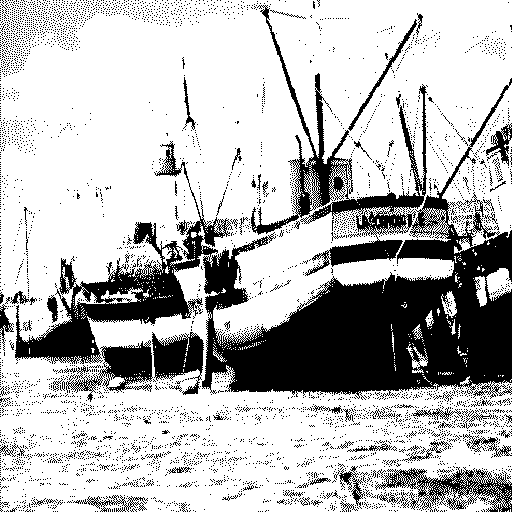
\includegraphics[width=.9\textwidth]{img/boat.png}}
        \caption{original}
    \end{subfigure}
    \hspace{2em}
    \begin{subfigure}[t]{\subfiguresize}\centering
        \fbox{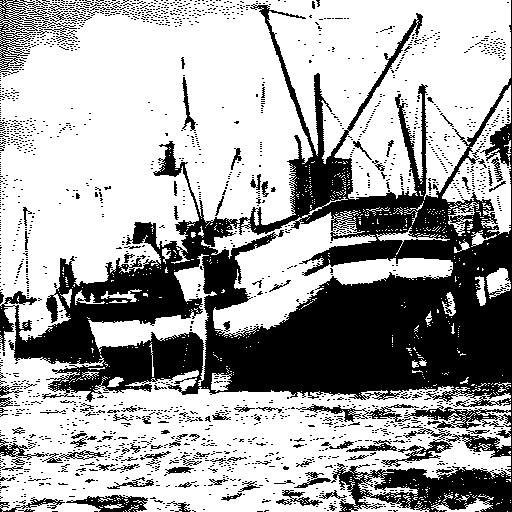
\includegraphics[width=.9\textwidth]{img/boat-erosion-b1.png}}
        \caption{$B_1$}
    \end{subfigure}
    \hspace{2em}
    \begin{subfigure}[t]{\subfiguresize}\centering
        \fbox{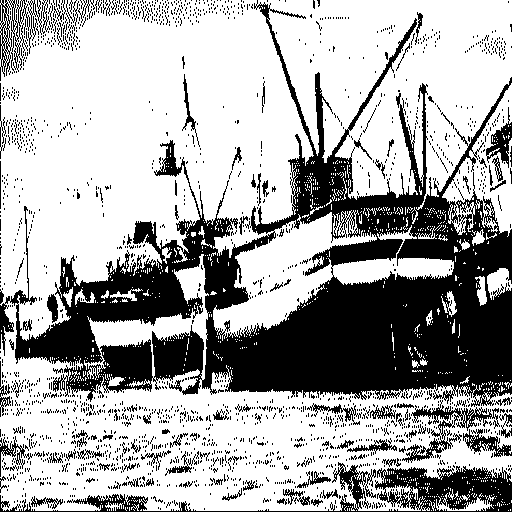
\includegraphics[width=.9\textwidth]{img/boat-erosion-b2.png}}
        \caption{$B_2$}
    \end{subfigure}\\[1em]
    \hspace{2em}
    \begin{subfigure}[t]{\subfiguresize}\centering
        \fbox{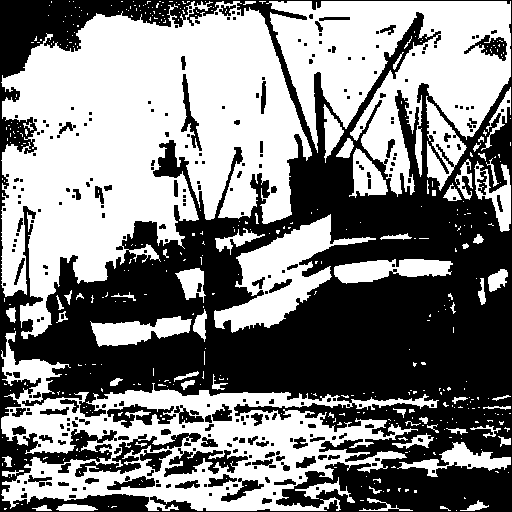
\includegraphics[width=.9\textwidth]{img/boat-erosion-b3.png}}
        \caption{$B_3$}
    \end{subfigure}
    \hspace{2em}
    \begin{subfigure}[t]{\subfiguresize}\centering
        \fbox{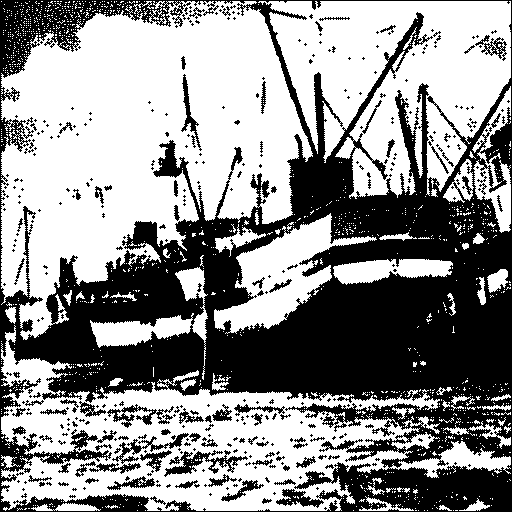
\includegraphics[width=.9\textwidth]{img/boat-erosion-b4.png}}
        \caption{$B_4$}
    \end{subfigure}
    \hspace{2em}
    \caption{Results of applying erosion on the boat image}
\end{figure} 

Similarly to dilation, the erosion is also a very simple operation so there is not much to say as conclusions.

All of the structuring elements had the effect that would be logically expected knowing the principle of erosion.
Kernel $B_1$ removed left-most pixels, whereas $B_2$ removed pixels from the bottom of the shape,
thus resulting in $B_1$ removing thin vertical lines, and $B_2$ removing thin horizontal lines.

As for kernels $B_3$ and $B_4$ the results look similar.
They both removed pixels from all of the sides of the image, with only difference that $B_3$ removed more pixels,
and $B_4$ being more subtle, leaving the result with less straight lines, overall looking more ``smooth'' for lack of a better word.

\subsection{Opening}

After applying the opening operation on 1-bit images the results are presented below.

\begin{figure}[H]\centering
    \begin{subfigure}[t]{\subfiguresize}\centering
        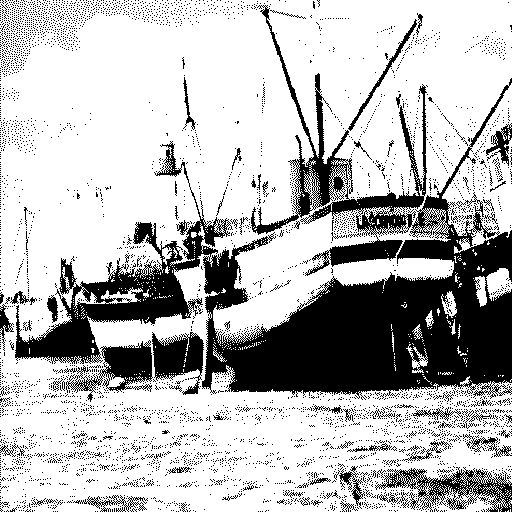
\includegraphics[width=\textwidth]{img/magda/boatbw.png}
        \caption{before}
    \end{subfigure}
    \hspace{2em}
    \begin{subfigure}[t]{\subfiguresize}\centering
         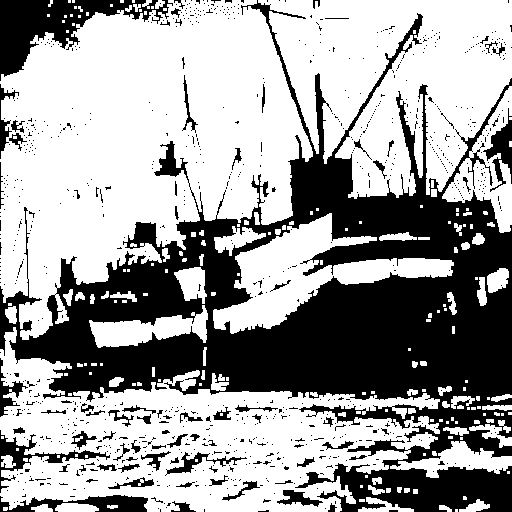
\includegraphics[width=\textwidth]{img/magda/output1.png}
        \caption{after}
    \end{subfigure}\\[1em]
    \begin{subfigure}[t]{\subfiguresize}\centering
        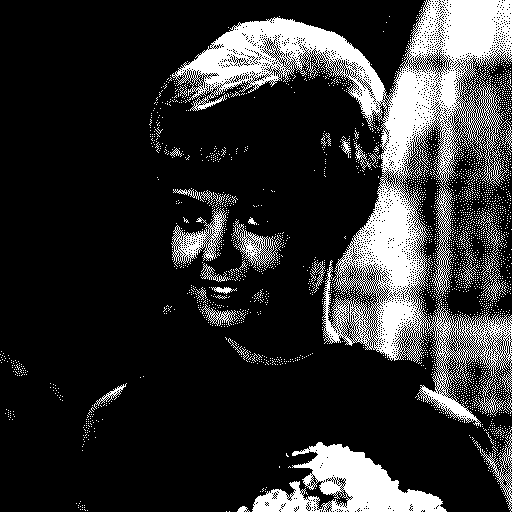
\includegraphics[width=\textwidth]{img/magda/girlbw.png}
        \caption{before}
    \end{subfigure}
    \hspace{2em}
    \begin{subfigure}[t]{\subfiguresize}\centering
         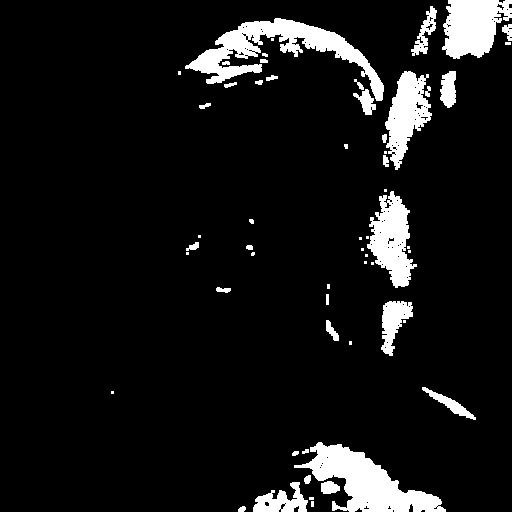
\includegraphics[width=\textwidth]{img/magda/output2.png}
        \caption{after}
    \end{subfigure}
    \caption{Results of applying opening operation with kernel $B_3$}
\end{figure}  

Based on the results of applying the opening operation, it is possible to draw the following conclusions. Firstly, the opening operation is effective at removing small objects from an image, such as noise or small unwanted details. Secondly, The shape of the structuring element used in the opening operation can influence the final result, with different shapes producing different levels of detail and overall image quality. It happened in the first, where those input images had either small unwanted details or noise. However, when applying opening operation on the second picture, the result came out as worse. It is hard to see the details and almost majority of the picture is black. 

Overall, the opening operation is a valuable tool in image processing, with a wide range of applications in fields such as computer vision and medical imaging.

\subsection{Closing}

After applying the closing operation on 1-bit images the results are presented below.

\begin{figure}[H]\centering
    \begin{subfigure}[t]{\subfiguresize}\centering
        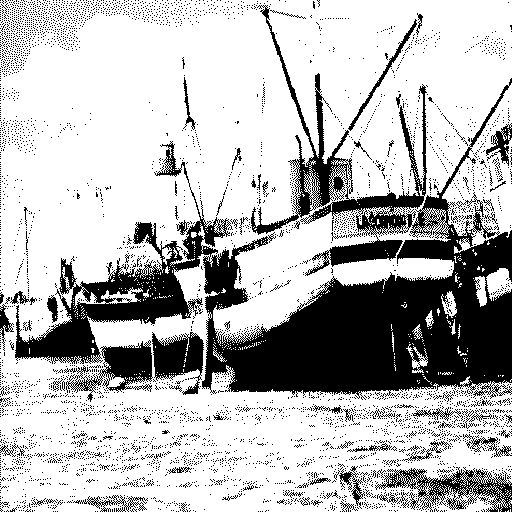
\includegraphics[width=\textwidth]{img/magda/boatbw.png}
        \caption{before}
    \end{subfigure}
    \hspace{2em}
    \begin{subfigure}[t]{\subfiguresize}\centering
         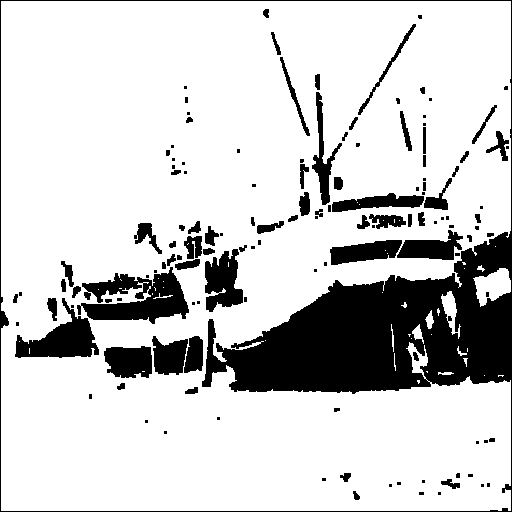
\includegraphics[width=\textwidth]{img/magda/output6.png}
        \caption{after}
    \end{subfigure}\\[1em]
    \begin{subfigure}[t]{\subfiguresize}\centering
        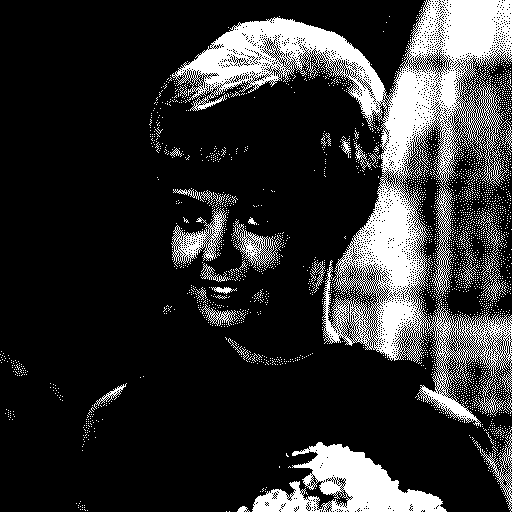
\includegraphics[width=\textwidth]{img/magda/girlbw.png}
        \caption{before}
    \end{subfigure}
    \hspace{2em}
    \begin{subfigure}[t]{\subfiguresize}\centering
         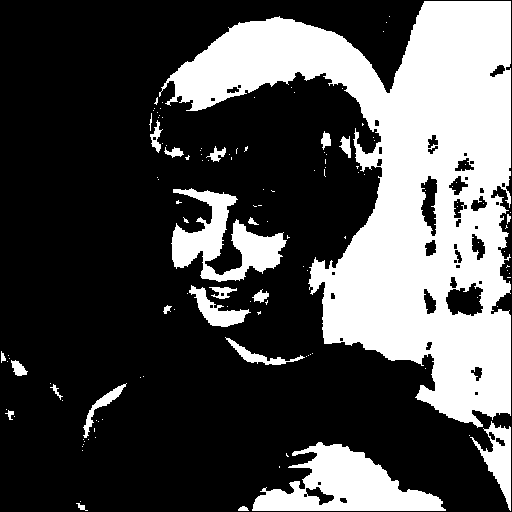
\includegraphics[width=\textwidth]{img/magda/output5.png}
        \caption{after}
    \end{subfigure}
    \caption{Results of applying closing operation with kernel $B_3$}
\end{figure}  

Based on the results of applying the opening operation, it is possible to draw the following conclusions. Firstly, The closing operation is effective at filling small holes or gaps in an image, such as those caused by noise or other types of image degradation. Secondly, The shape of the structuring element used in the closing operation can influence the final result, with different shapes producing different levels of detail and overall image quality. Contrary to the opening result images, the first image came out as worse and the second picture came out as better. The woman in the second picture thanks to closing operation has more visually noticeable details  on her face. The first and last picture however lost all the details and it is hard to notice anything from them.

Overall, the closing operation is a valuable tool in image processing, with the same usefulness in computer vision and medical imaging just like opening operation.
\subsection{Hit-or-miss transform}

For testing the \textsc{hmt}, we came up with a mask, that should detect right edges of the shape.
If they are in fact detected, we will know that the \textsc{hmt} works correctly.

In addtion, the \textsc{hmt} will be tested much more, while analyzing the convex hull in sec.~\ref{sec:convex-hull-analysis}.

\begin{figure}[H]\centering
    \begin{tikzpicture}[baseline=(A.base)]
        \matrix[square matrix]
        {
        &  & \\
        & |[fill=green]|$\odot$ & |[fill=red]| \\
        & & \\
        };
    \end{tikzpicture}
    \caption{The structuring element used for testing the \textsc{hmt}.}
\end{figure}

\begin{figure}[H]\centering
    \begin{subfigure}[t]{\subfiguresize}
        \includegraphics[width=\textwidth]{img/image1.png}
        \caption{original}
    \end{subfigure}
    \hspace{2em}
    \begin{subfigure}[t]{\subfiguresize}
        \includegraphics[width=\textwidth]{img/hmt-left.png}
        \caption{after \textsc{hmt}}
    \end{subfigure}\\[1em]
    \begin{subfigure}[t]{\subfiguresize}
        \includegraphics[width=\textwidth]{img/image2.png}
        \caption{original}
    \end{subfigure}
    \hspace{2em}
    \begin{subfigure}[t]{\subfiguresize}
        \includegraphics[width=\textwidth]{img/hmt2-left.png}
        \caption{after \textsc{hmt}}
    \end{subfigure}
\end{figure}

As we can see in the above figure, the right edges of the shape were succesfully detected.
Therefore we conclude that the \textsc{hmt} works correctly.

\section{Description of the implementation of the assigned variant of morphological algorithm}

\subsection{Description}
The algorithm we had to implement is the convex hull.

It is used to eliminate any concavities from the shape.
The calculation of a convex hull of some image $A$ works as follows:

For each structuring element $\mathbf{B}^i$ from elements shown on fig. \ref{fig:convex-hull-kernels},
we repeatedly apply the \textsc{hmt}, until there is no change.

For calculating the subsequent iterations of applying the HMTs, we have formula
\begin{equation}
    X^i_k = (X^i_{k-1} \otimes \mathbf{B}^i) \cup A
    \label{eq:convex-hull-iteration-err}
\end{equation}
Our starting condition is
\begin{equation}
    X^i_0 = A
    \label{eq:convex-hull-start-condition}
\end{equation}
We apply equation (\ref*{eq:convex-hull-iteration-err}) until we find the smallest $k$ such that:
\begin{equation}
    X^i_k = X^i_{k-1}
    \label{eq:convex-hull-final-condition}
\end{equation}

When we reach the final condition, we yield the result $X^i_k$ as $D^i$.

The final result of the computation is the union of all $D^i$ for all $i$.

\begin{figure}[H]\centering
    \begin{subfigure}[t]{.2\textwidth}\centering
        \begin{tikzpicture}
            \matrix[square matrix]
            {
            |[fill=green]|&&\\
            |[fill=green]|&|[fill=red]|$\odot$&\\
            |[fill=green]|&&\\
            };
        \end{tikzpicture}
        \caption{$\mathbf{B}^1$}
        \label{kernel-convex-left}
    \end{subfigure}
    \begin{subfigure}[t]{.2\textwidth}\centering
        \begin{tikzpicture}
            \matrix[square matrix]
            {
            |[fill=green]|&|[fill=green]|&|[fill=green]|\\
            &|[fill=red]|$\odot$&\\
            &&\\
            };
        \end{tikzpicture}
        \caption{$\mathbf{B}^2$}
        \label{kernel-convex-up}
    \end{subfigure}
    \begin{subfigure}[t]{.2\textwidth}\centering
        \begin{tikzpicture}
            \matrix[square matrix]
            {
            &&|[fill=green]|\\
            &|[fill=red]|$\odot$&|[fill=green]|\\
            &&|[fill=green]|\\
            };
        \end{tikzpicture}
        \caption{$\mathbf{B}^3$}
        \label{kernel-convex-right}
    \end{subfigure}
    \begin{subfigure}[t]{.2\textwidth}\centering
        \begin{tikzpicture}
            \matrix[square matrix]
            {
            &&\\
            &|[fill=red]|$\odot$&\\
            |[fill=green]|&|[fill=green]|&|[fill=green]|\\
            };
        \end{tikzpicture}
        \caption{$\mathbf{B}^4$}
        \label{kernel-convex-down}
    \end{subfigure}
    \caption{Structuring elements used for convex hull}
    \label{fig:convex-hull-kernels}
\end{figure}

\pagebreak[3 ]
\subsection*{The error in the formula}

If the task was to be followed exactly as given in the instruction, it would not yield the desired result.
To be precise, for all $\mathbf{B}^i$ in fig. \ref{fig:convex-hull-kernels}, for any image $A$:
\begin{equation*}
    (A \otimes \mathbf{B}^i) \neq \emptyset \implies \mbox{\large$\mathsurround0pt\nexists$} D^i
\end{equation*}

\begin{proof}
    In all of the structuring elements in fig.~\ref{fig:convex-hull-kernels}, the origin (marked $\odot$) is marked as `miss', meaning, that it must not be present in the original image.
    As a consequence of that:
    \begin{equation}
        \biggerforall\nolimits_i\biggerforall\nolimits_k \; X^i_k \cap (X^i_k \otimes \mathbf{B}^i) = \emptyset
        \label{eq:convex-hull-disjoint-hmt}
    \end{equation}

    Now, if we substitute the final condition (\ref{eq:convex-hull-final-condition}) to eq.~(\ref{eq:convex-hull-iteration-err}), we get:
    \begin{equation}
        X^i_k = (X^i_k \otimes \mathbf{B}^i) \cup A
        \label{eq:convex-hull-iteration-error-substituted}
    \end{equation}

    Applying $X = X \cap X$, we get
    \begin{align}
        X^i_k & = X^i_k \cap \big((X^i_k \otimes \mathbf{B}^i) \cup A \big) \nonumber    \\
              & = \big(X^i_k \cap (X^i_k \otimes \mathbf{B}^i) \big) \cup (X^i_k \cap A)
    \end{align}

    Applying eq.~(\ref{eq:convex-hull-disjoint-hmt})
    \begin{align}
        X^i_k & = \emptyset \cup (X^i_k \cap A) \nonumber \\
              & = X^i_k \cap A \nonumber                  \\
              & = A \label{eq:convex-hull-only-zero-k}
    \end{align}
    Which is the same as eq.~(\ref{eq:convex-hull-start-condition}), so $k=0$.\\
    Finally, substituting this equation to eq.~(\ref{eq:convex-hull-iteration-error-substituted}), we get
    \begin{equation}
        A = (A \otimes \mathbf{B}^i) \cup A
    \end{equation}

    Which is true if and only if $(A \otimes \mathbf{B}^i) \subseteq A$.\\
    Since $(A \otimes \mathbf{B}^i) \subseteq A$ and from eq.~\eqref{eq:convex-hull-disjoint-hmt}, $(A \otimes \mathbf{B}^i) \cap A = \emptyset$, we have:
    \begin{equation}
        (A \otimes \mathbf{B}^i) = \emptyset
    \end{equation}
    Therefore,
    \begin{align*}
        \bigexists k                              & \iff (A \otimes \mathbf{B}^i) = \emptyset    \\
        \mbox{\large$\mathsurround0pt\nexists$} k & \iff (A \otimes \mathbf{B}^i) \neq \emptyset
    \end{align*}
    Since $\nexists k \Rightarrow \nexists D^i$, we have
    \begin{equation}
        (A \otimes \mathbf{B}^i) \neq \emptyset \implies \mbox{\large$\mathsurround0pt\nexists$} D^i
    \end{equation}
\end{proof}

As the above shows, there are two possibilities of running the algorithm:
\begin{enumerate}
    \item If $\bigforall_i \; (A \otimes \mathbf{B}^i) = \emptyset$, then all $k = 0$ and algorith returns the original image unchanged
    \item Else, the algorithm gets stuck in the infinite loop trying to find $k$ that does not exist
\end{enumerate}

Therefore, we concluded that for the algorithm to work as expected, we must change the eq.~\eqref{eq:convex-hull-iteration-err} to the following:
\begin{equation}
    X^i_k = (X^i_{k-1} \otimes \mathbf{B}^i) \cup X^i_{k-1}
\end{equation}

Now, $k$ will always exist, and it will be such $k$ that $(X^i_k \otimes \mathbf{B}^i) = \emptyset$.

\pagebreak[2]
\subsection{Implementation}
\label{sec:convex-hull-impl}

The implementation can be split into 2 distinct parts.
The first one is calculating $D^i$ for a given $\mathbf{B}^i$.
We will refer to this step as ``saturating'' the image with the hit-or-miss transformation.
The second step is merging all of the resulting images into one.

With standard implementation, we would have to loop over the entire image to calculate the \textsc{hmt}.
Then, we would need to loop again to perform the image union with $X^i_{k-1}$.
This would have to be performed $k$ times for each structuring element.
Finally we would have to loop over the entire image once again to merge all of $D^i$.

However, we are able to perform major optimization by removing the need of applying the union altogether.
We can acomplish this by, instead of using standard \textsc{hmt}, making use of the abovementioned function that returns an iterator to all of the pixels that fullfill the \textsc{hmt} conditions.
We do this by not allocating a clear image buffer for the output of \textsc{hmt}, but instead output the result directy to the image in place.
This firstly, reduces the number of operations significantly, and secondly, drastically reduces the memory complexity, as we will not allocate any aditional buffers.

This also applies to union of $D^i$, because we can redefine the initial conditions from eq.~\eqref{eq:convex-hull-final-condition} as the following:
\begin{equation*}
    X^i_0 =
    \begin{cases}
        A       & \text{for $i = 0$}, \\
        D^{i-1} & \text{for $i > 0$}
    \end{cases}
\end{equation*}

\pagebreak[2]
Below is our implementation of this algorithm:
\begin{lstlisting}
for (hit, miss) in &STRUCTURAL_ELEMENTS {
    let transform = 
        HitOrMissTransform::new(hit.clone(), miss.clone());

    loop {
        let transform_result: Vec<_> = 
            transform.get_matching_pixels(image).collect();
        if transform_result.len() == 0 {
            break;
        }
        for (x, y) in transform_result {
            image.put_pixel(x, y, FOREGROUND_PIXEL);
        }
    }
}
\end{lstlisting}

\section{Analysis of the results of the assigned variant of morphological algorithm}
\label{sec:convex-hull-analysis}

The results of applying the convex hull are presented below:

\begin{figure}[h]\centering
    \begin{subfigure}[t]{\subfiguresize}
        \includegraphics[width=\textwidth]{img/image1.png}
        \caption{before}
    \end{subfigure}
    \hspace{2em}
    \begin{subfigure}[t]{\subfiguresize}
        \includegraphics[width=\textwidth]{img/image1-convexhull.png}
        \caption{after}
    \end{subfigure}\\[2em]

    \begin{subfigure}[t]{\subfiguresize}
        \includegraphics[width=\textwidth]{img/image2.png}
        \caption{before}
    \end{subfigure}
    \hspace{2em}
    \begin{subfigure}[t]{\subfiguresize}
        \includegraphics[width=\textwidth]{img/image2-convexhull.png}
        \caption{after}
    \end{subfigure}
    \caption{Result of applying the convex hull}
\end{figure}

As we can see, the convex hull worked as expected, eliminating any concavities in the input shape.
It procuded a diagonal rectangle, completely containing the original shape.
The downside of the algorithm is that it often outputs more pixels that are actually needed for the shape to be convex.

For testing we chose custom shapes, prepared in such a way, that has a diagonal skeleton, while the other has an orthogonal one.
The algorithm yielded much better result for the othogonal-based shape, 
because it outputs less unnecessary pixels.

This behaviour is to be expected, because the choice of the structuring elements on fig. \ref{fig:convex-hull-kernels}, 
is such, that the algorithm will expand the shape in the orthogonal directions.
Therefore, the resulting shape will be rectangle composed of $45^\circ$-rotated lines.

As a consequence, the dimensions of output shape will be dictated by the maximum taxicab distance from the corners of the image.

That is, let $C$ be the set of the corners of an image:
\begin{equation*}
    C = \big\{ (0,0),\, (x_{max},0),\, (y_{max},0),\, (x_{max},y_{max}) \big\}
\end{equation*}
Then, if $A$ is the image before applying convex hull, and $A'$ is after:
\begin{equation*}
    \biggerforall_{(x_0,y_0) \in C} \;
    \max\limits_{(x,y) \in A}\Big\{ |x - x_0| + |y - y_0| \Big\} = \max\limits_{(x,y) \in A'} \Big\{ |x - x_0| + |y - y_0| \Big\}
\end{equation*}

Therefore, although the diagonal and orthogonal shapes have the similar dimensions in the sense of euclidean geometry,
in taxicab distance, the orthogonal shape will have much smaller dimensions, and thus, much smaller dovex hull.

If, however, instead of structuring elements from fig. \ref{fig:convex-hull-kernels}, 
we used such elements, that the image would expand diagonally, thus producing convex hull in the shape of an orthogonal rectangle,
we would find that the dimensions of the hull are determined by the dimensions of the shape in terms of the chebyshev distance,
thus yielding better results for the diagonal shape.

\section{Description of the implementation of the assigned segmentation variant}
\subsection{Description}
Region growing is a type of image segmentation technique that is used to identify and separate different objects or regions within an image. It works by starting from a seed point within an image and then iteratively expanding the region by adding adjacent pixels that meet certain criteria, such as being within a certain range of intensity or color.

To perform region growing, the image is first divided into a set of small, connected regions, or seeds. Each seed represents a potential region within the image, and the algorithm starts by selecting one of these seeds as the starting point for region growing. The algorithm then compares the values of the pixels in the seed to the values of the pixels in the surrounding area. If the values of the surrounding pixels meet certain criteria, such as being within a certain range of intensity or color, they are added to the growing region. This process is repeated until all adjacent pixels have been examined, at which point the region is complete.

Region growing is useful for separating objects or regions within an image that have similar characteristics, such as intensity or color. It is a popular technique in image processing because it is relatively simple to implement and can be used to segment images of various types, including binary, grayscale, and color images.

Our implementation uses a breadth-first search algorithm to expand the region from the seed point. It maintains a queue of pixels to visit and adds the neighboring pixels of each pixel to the queue if they have a similar intensity value to the seed point, within a specified tolerance. The resulting image is a binary image with the region of interest marked in white and the rest of the image marked in black. For the images in color, the program takes only the first channel - red for processing the image.

\subsection{Implementation}

In our implementation, \lstinline{seed_x} and \lstinline{seed_y} represent the $x$ and $y$ coordinates respectively,
of the seed point in the image chosen by the user.
The seed point is also the starting point for the region growing algorithm.
The \lstinline{tolerance} is also chosen by the user.
Firstly, we are checking whether the chosen pixel is within the dimensions of the input image.
If the seed point is within the image dimensions,
the transformation for region growing can be performed.
Below the implementation of the \lstinline{Transformation} trait for \lstinline{RegionGrowing}:

\begin{lstlisting}
    
impl Transformation for RegionGrowing {
    fn apply(&self, image: &mut RgbImage) {
        if self.seed_x.get() >= image.width() {
            self.seed_x.set(image.width() - 1);
        }
        if self.seed_y.get() >= image.height() {
            self.seed_y.set(image.height() - 1);
        }
        let seed_pixel = 
        image.get_pixel(self.seed_x.get(), self.seed_y.get());
        let mut new_image: GrayImage = 
        ImageBuffer::new(image.width(), image.height());
        let mut queue = VecDeque::new();
        queue.push_back((self.seed_x.get(), self.seed_y.get()));

        while let Some((x, y)) = queue.pop_front() {
            if x >= image.width() || y >= image.height() {
                continue;
            }
            let pixel = image.get_pixel(x as u32, y as u32);
            let new_image_pixel = new_image.get_pixel(x as u32, y as u32);

            if new_image_pixel[0] == 
            0 && is_similar(pixel, seed_pixel, self.tolerance) {
                new_image.put_pixel(x as u32, y as u32, Luma([255]));

                queue.push_back((x + 1, y));
                queue.push_back((x, y + 1));
                if x > 0 {
                    queue.push_back((x - 1, y));
                }
                if y > 0 {
                    queue.push_back((x, y - 1));
                }
            }
        }

        *image = DynamicImage::from(new_image).to_rgb8();
    }
}
*image = DynamicImage::from(new_image).to_rgb8();
\end{lstlisting}

The \lstinline{is_similar} function was implemented by taking in a reference to a pixel
and a reference to a seed pixel,
as well as a tolerance value.
It calculates the difference between the value of the pixel
and the seed pixel and returns true if the difference is less than or equal
to the tolerance value. Below the implementation of the \lstinline{is_similar} function:

\begin{lstlisting}
fn is_similar(pixel: &Rgb<u8>, seed_pixel: &Rgb<u8>, tolerance: u8) 
-> bool {
    let diff: i16 = 
    (pixel[0] as i16 - seed_pixel[0] as i16).abs() as i16;
    diff <= tolerance as i16
}
\end{lstlisting}

\section{Analysis of the results of the assigned segmentation variant}

The results of applying the region merging are presented below:

\begin{figure}[H]\centering
    \begin{subfigure}[t]{\subfiguresize}
        \includegraphics[width=\textwidth]{img/magda/boat.png}
        \caption{before}
    \end{subfigure}
    \hspace{2em}
    \begin{subfigure}[t]{\subfiguresize}
        \includegraphics[width=\textwidth]{img/magda/region_output.png}
        \caption{after}
    \end{subfigure}\\[2em]

    \begin{subfigure}[t]{\subfiguresize}
        \includegraphics[width=\textwidth]{img/magda/camera.png}
        \caption{before}
    \end{subfigure}
    \hspace{2em}
    \begin{subfigure}[t]{\subfiguresize}
        \includegraphics[width=\textwidth]{img/magda/region_output2.png}
        \caption{after}
    \end{subfigure}
    \caption{Result of applying region merging of a chosen randomly pixel (100,100) and tolerance of 100 on 8-bits gray scale images}
\end{figure}

\begin{figure}[H]\centering
    \begin{subfigure}[t]{\subfiguresize}
        \includegraphics[width=\textwidth]{img/magda/girlbw.png}
        \caption{before}
    \end{subfigure}
    \hspace{2em}
    \begin{subfigure}[t]{\subfiguresize}
        \includegraphics[width=\textwidth]{img/magda/region_output_new1.png}
        \caption{after}
    \end{subfigure}\\[2em]
    \caption{Result of applying region merging of a chosen randomly pixel (100,100) and tolerance of 100 on 1-bit binary image}
\end{figure}

\begin{figure}[H]\centering
    \begin{subfigure}[t]{\subfiguresize}
        \includegraphics[width=\textwidth]{img/magda/girlc.png}
        \caption{before}
    \end{subfigure}
    \hspace{2em}
    \begin{subfigure}[t]{\subfiguresize}
        \includegraphics[width=\textwidth]{img/magda/region_output_new2.png}
        \caption{after}
    \end{subfigure}\\[2em]
    \caption{Result of applying region merging of a chosen randomly pixel (100,100) and tolerance of 100 on 24-bits color image}
\end{figure}

As we can clearly see, depending on a user input, the output picture can change. In both cases, the program did indeed 'merged' pixels of the same value and produced the pictures above. Overall, the success of a region merging operation will depend on the specific input of the data by a user and an input image. By carefully selecting appropriate criteria for merging and carefully evaluating the results, it is possible to achieve good results with region merging in many image processing applications.

The results of a region merging operation can be evaluated in a number of ways. One common metric is the mean squared error (MSE) between the original image and the merged regions. This can be used to measure the accuracy of the region merging operation and to identify any artifacts or distortions that may have been introduced. 

There are various homogeneity criteria that can be used to determine whether two regions should be merged or not. Firstly, the intensity homogeneity. This criterion involves merging regions that have similar intensity values, i.e., the average intensity of the pixels in each region is similar. This can be useful for segmenting objects with uniform color or brightness. In our project we chose the approach of intensity-based region growing, which involves in adding pixels to the region based on their intensity/gray level values. Secondly, color homogeneity. This criteria involves merging regions that have similar color values, i.e., the average color of the pixels in each region is similar. This can be useful for segmenting objects with uniform color or for separating different colors in an image. And thirdly, texture homogeneity. This criteria involves merging regions that have similar texture patterns, i.e., the spatial distribution of intensity or color values in each region is similar. This can be useful for segmenting objects with distinct texture patterns, such as wood grain or fabric.

There are visual differences when analysing the result images of region merging. Those input values used for this experiment are random. However, choosing the right seed pixel and smaller tolerance might result in better looking pictures for a user. Those presented above are only experimental for the analysis with the same parameters. 

Overall, the effectiveness of region merging in image processing depends on the specific task and the desired output. Choosing the appropriate homogeneity criteria and algorithm parameters can help improve the accuracy and efficiency of the operation.


\section{Description of other changes which took place in the application}

Using the console interface proved to be very tedious to use for a long time,
especially with repeated transformations and long filepaths.
Additionally, to view the results, we would have to save to external file and open it every time.

To make things more easy to use, we started work on a graphical user interface for our project.

This was pretty straightforward to set up, as all of our image operations were in form of a static library, 
decoupled from the console interface. 
Thus, it was just a matter of creating another binary with a reference to our image operations.

For the framework, we decided to try Tauri (see \href{https://tauri.app/about/intro}{tauri webpage}), which is similar to elecron, with the key difference that has better performance, and smaller executable size.
The backend code is written in Rust, and consists mostly of calling our image operations library,
and the frontend is done using Svelte (see \href{https://svelte.dev}{svelte webpage}) with typescript.

So far, we were only able to implement some of the transformations from the previous tasks,
but with some free time we might expand the functionality in the future.

\begin{figure}[H]\centering
    \includegraphics[width=.8\textwidth]{gui_screenshot.png}
    \caption{Graphical user interface for our image processing application}
\end{figure}

\end{document}